\section{Architecture} \label{sect:case-study:arch}

% Introduction to overall architecture 
The following section motivates and outlines the architecture choices made in order to create the tools required to conduct the case study. The software required to perform the case study is split into two independent applications. The first application focuses in user interaction and experience, referred to as the \mlblinkui, and the second one is in charge of dealing with domain logic and providing the required resources to the \mlblinkui, referred to as the \mlblinkapi. Through out the report, these two applications are also described as the client and server respectively.  \newline

% Why two separate applications?
While the two applications could have been developed as a monolith, having two decoupled applications allows to clearly distinguish between client responsibilities and domain logic. This approach also allows to support multiple types of clients such as WEB, mobile, and desktop -- all using the \mlblinkapi to handle domain logic, as well as simpler delegation in the sense that a person(s) which only needs to work on the client will not need to setup the server dependencies; this person(s) can simply connect the local \mlblinkui to a development instance of the \mlblinkapi running in the cloud. \newline

On the other hand, splitting the project into two separate applications comes with a higher operational overhead. For instance, deploying a new feature could require rolling out a new version of both the client and the server, while taking into account that and older version of the client might be cached in the user's browser. Figure \ref{fig:ml-blink-architecture} shows a summary of how the \mlblinkui, \mlblinkapi, and a user depicted by a computer interact with each other.

\begin{figure}
  \centering
  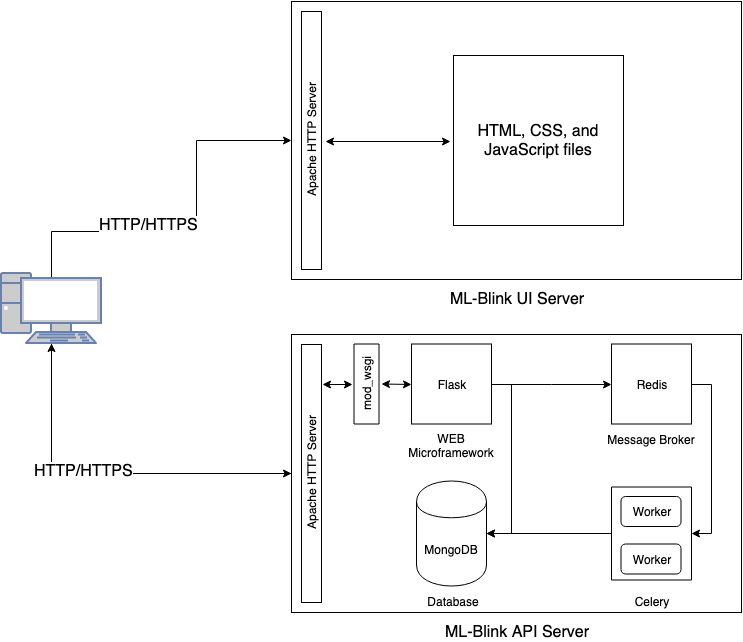
\includegraphics[
        width=\textwidth,
        height=\textheight,
        keepaspectratio
  ]{report/images/ml-blink-architecture.png}
  \caption{Summary of how the \mlblinkui and the \mlblinkapi interact with each other when used by a client depicted by a computer in this scenario.}
  \label{fig:ml-blink-architecture}
\end{figure}